% \subfloat[Unstructured data]{%
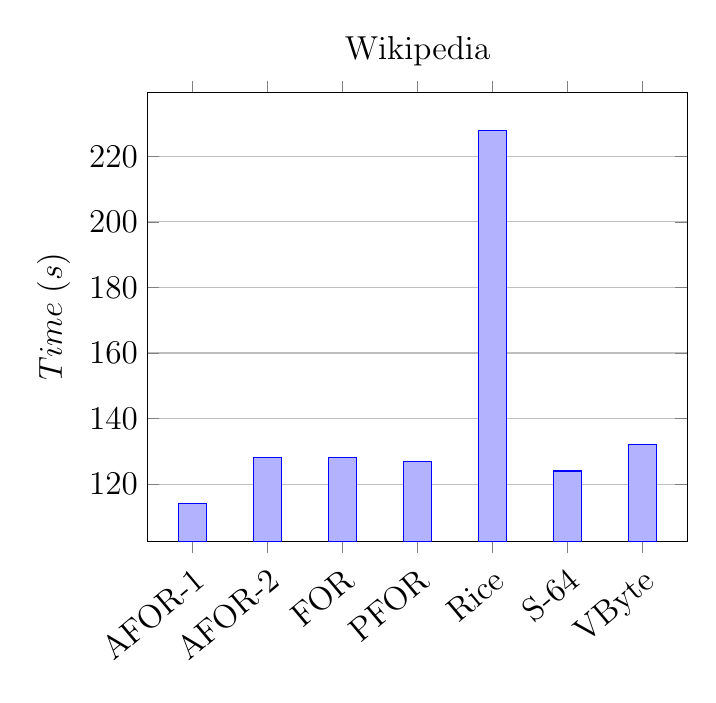
\begin{tikzpicture}[baseline]
\begin{axis}[
ylabel=$Time \; (s)$,
x tick label style={rotate=40, anchor=north east},
xtick={1,...,7},
xticklabels={AFOR-1, AFOR-2, FOR, PFOR, Rice, S-64, VByte},
legend style={at={(0.5,1.13)}, anchor=north, legend columns=-1},
label style={font=\large},
tick label style={font=\large},
title style={font=\large},
ybar,
ymajorgrids=true,
bar width=10pt,
title={Wikipedia},
%enlargelimits=0.15,
]
\addplot
coordinates {(1, 114) (2, 128) (3, 128) (4, 127) (5, 228) (6, 124) (7, 132)};
\end{axis}
\end{tikzpicture}%
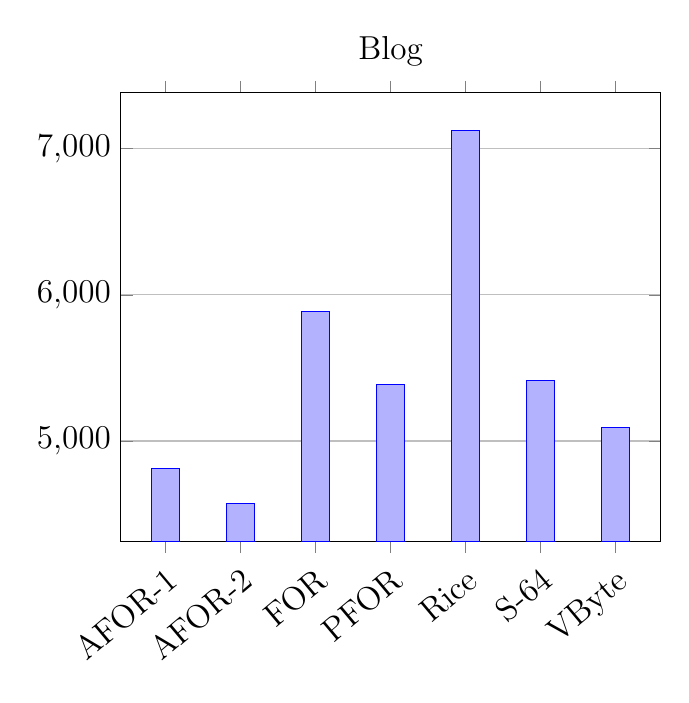
\begin{tikzpicture}[baseline]
\begin{axis}[
x tick label style={rotate=40, anchor=north east},
xtick={1,...,7},
xticklabels={AFOR-1, AFOR-2, FOR, PFOR, Rice, S-64, VByte},
legend style={at={(0.5,1.13)}, anchor=north, legend columns=-1},
label style={font=\large},
tick label style={font=\large},
title style={font=\large},
ybar,
ymajorgrids=true,
bar width=10pt,
title={Blog},
%enlargelimits=0.15,
]
\addplot
coordinates {(1, 4813) (2, 4571) (3, 5888) (4, 5387) (5, 7127) (6, 5414) (7,
5092)};
\end{axis}
\end{tikzpicture}
% }